\documentclass[12pt,oneside]{article}
\usepackage{geometry}                                % See geometry.pdf to learn the layout options. There are lots.
\usepackage{listings}				% Permite utilizar lenguajes de programacion dentro de latex
\geometry{a4paper}                                           % ... or a4paper or a5paper or ... 
%\geometry{landscape}                                % Activate for for rotated page geometry
%\usepackage[parfill]{parskip}                    % Activate to begin paragraphs with an empty line rather than an indent
\usepackage{graphicx}                                % Use pdf, png, jpg, or epsß with pdflatex; use eps in DVI mode
                                                                % TeX will automatically convert eps --> pdf in pdflatex                
\usepackage{amssymb}

\usepackage[spanish]{babel}                        % Permite que partes automáticas del documento aparezcan en castellano.
\usepackage[utf8]{inputenc}                        % Permite escribir tildes y otros caracteres directamente en el .tex
\usepackage[T1]{fontenc}                                % Asegura que el documento resultante use caracteres de una fuente apropiada.

\usepackage{hyperref}                                % Permite poner urls y links dentro del documento
\usepackage{listings}

\title{Ejercicios de Programación - Sebesta}
\author{Lenguajes de Programación - ESPOL}

%\date{}                                                        % Activate to display a given date or no date

\begin{document}
\maketitle

	\section{Introducción}
	Las respuestas propuestas en este repositorio son producto del trabajo de los estudiantes de la materia ``Lenguajes de Programación'' de la ESPOL, correspondientes a las preguntas del libro de Robert Sebesta, Concepts of Programming Languages.

	\section{Preguntas y Respuestas}

		\subsection{Capítulo 5: Nombres, Enlaces y Alcances}
			\begin{itemize}
				\item {\bf Pregunta 4: Write a Python function that has subprograms nested three deep and in which each nested subprogram references variables defined in all of its enclosing subprogram}	
					\begin{center}
						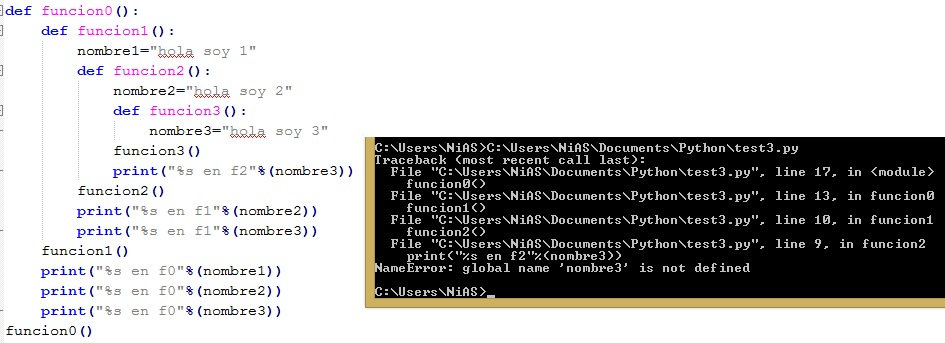
\includegraphics[scale=0.5]{Imagenes/6.jpg}\\
						NO EJECUTADO EN PYTHON: Variables no son declaradas globales
					\end{center}

				\item {\bf Pregunta 5: Write a C function that includes the following sequence of statements: x = 21;int x;x = 42; Run the program and explain the results. Rewrite the same code in C++ and Java and compare the results.}
					\begin{itemize}
						\item {Función en C}
							\begin{center}
							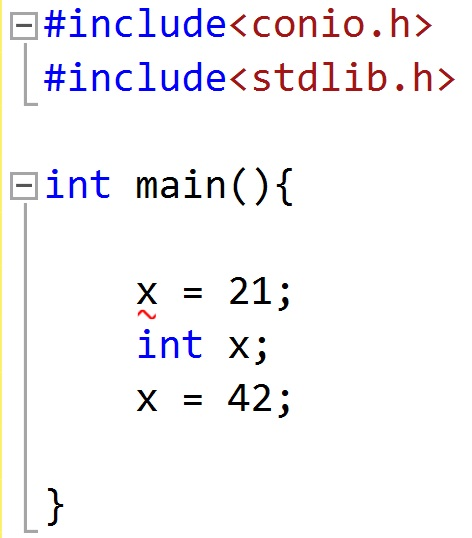
\includegraphics[scale=0.3]{Imagenes/1.jpg}\\
							NO COMPILA: error C2065: 'x' : identificador no declarado
							\end{center}
							ARGUMENTO: En el lenguaje C es necesario crear la variable o instanciarla de las siguientes formas antes de poder usarla o asignarle un valor: 
							\begin{itemize}
								\item{(tipo) (nombreVariable);}
									\\Ejemplo: int x;
								\item{(tipo) (nombreVariable)=(valor Inicial);}		
									\\Ejemplo: int x=10;							
							\end{itemize}

						\item {Función en C++}
							\\Sucede lo mismo que en C, el compilador de visual presenta los mismos errores, como si las tres lineas estuvieran mal escritas, aunque realmente es la primera.

						\item {Función en Java}
							\begin{center}
							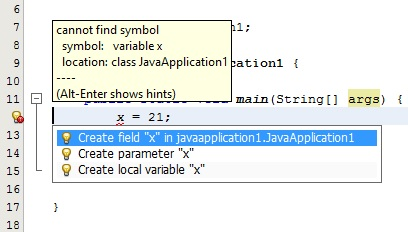
\includegraphics[scale=0.9]{Imagenes/2.jpg}\\
							NO COMPILA: error: cannot find symbol
							\end{center}		
							ARGUMENTO: En el lenguaje Java, el intérprete antes de compliar sugiere al programador crear la variable X como una variable de clase, y una vez compilado muestrar el error de que no puede encontrar el simbolo que se esta 									intentado usar, en este caso X.									
					\end{itemize}

				\item {\bf Pregunta 6: Write test programs in C++, Java, and C\# to determine the scope of a variable declared in a for statement. Specifically, the code must determine whether such a variable is visible after the body of the for statement.}
					\begin{itemize}
						\item {Función en C++}
							\begin{center}
								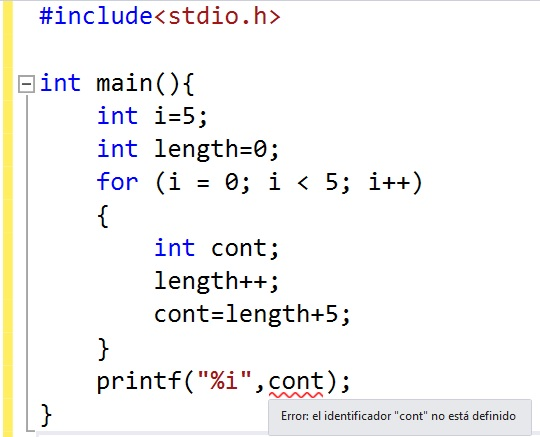
\includegraphics[scale=0.6]{Imagenes/3.jpg}\\
								NO COMPILA: No es visible despues de la sentencia for.
							\end{center}
						\item {Función en C\#}
							\begin{center}
								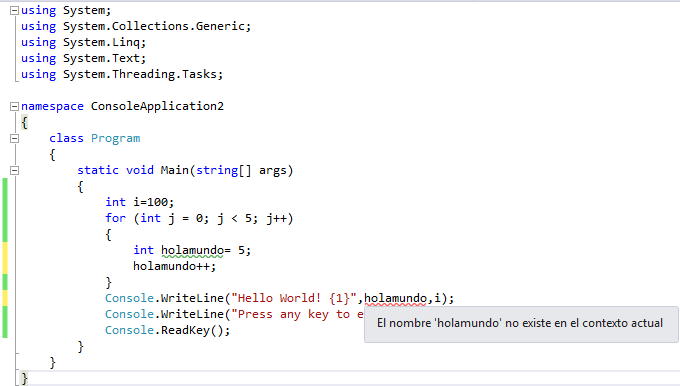
\includegraphics[scale=0.7]{Imagenes/4.jpg}\\
								NO COMPILA: No es visible despues de la sentencia for.
							\end{center}
							Es de notar que los avisos que muestra el intérprete son diferentes en los dos casos anteriores, en C++ nos dice que no existe definición de la variable que se quiere usar y por tanto no hay ningún valor que mostrar. En la 									siguiente, en C\# en cambio nos informa que no estamos en el mismo contexto y que por tanto la variable no es visible ni alcanzable.
					\end{itemize}
				\item {\bf Pregunta 7: Write three functions in C or C++: one that declares a large array statically, one that declares the same large array on the stack, and one that creates the same large array from the heap. Call each of the subprograms a large 					number of times (at least 100,000) and output the time required by each. Explain the results.}	
					\begin{center}
						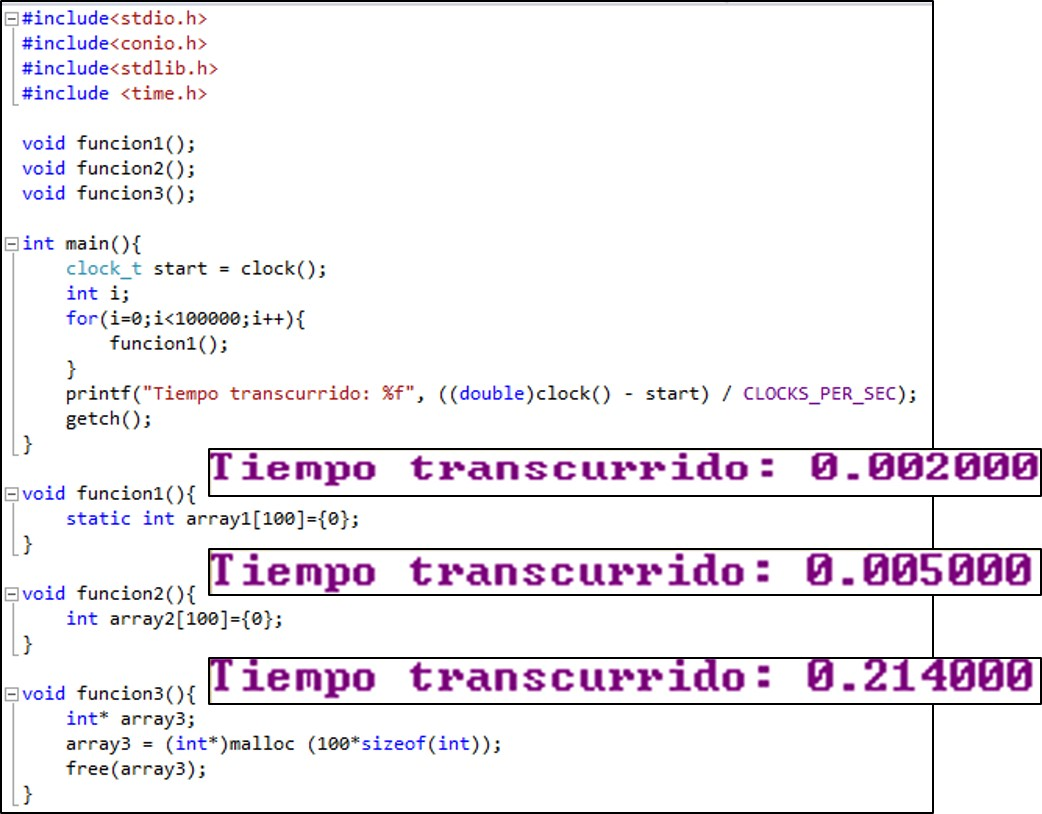
\includegraphics[scale=0.6]{Imagenes/5.jpg}\\
						EN C: Diferentes tiempos para diferentes funciones
					\end{center}
					ARGUMENTO: Las variables y vectores en C ocupan un tamaño fijo, el cuál es establecido antes de ejecutar el programa, por tanto no pueden variarlo durante esta ejecución. Por medio de punteros se puede reservar o liberar memoria 							dinámicamente, es decir, según se necesite. La Función malloc sirve para solicitar un bloque de memoria del tamaño suministrado como parámetro.
					Es notable que la petición MALLOC al querer reservar memoria toma más tiempo en su ejecución, pero también es importante entender que es una forma segura de programar, ya que estaremos seguros de que obtendremos la memoria que 							necesitemos para las variablemos que usemos, sin tener errores de memoria en tiempo de ejecución.
					Así que aunque en la imagén veamos que toma más tiempo ejecutar MALLOC es preferible su uso, para no arriesgarnos a errores de memoria.
		\end{itemize}


		\subsection{Capítulo 6: Tipos de Datos}
			\begin{itemize}
				\item {\bf Pregunta 1}
					OJOOOOOOOOOO faltaaaaaaaaaaaaaaaaaaaaa
				\item {\bf Pregunta 2}
					OJOOOOOOOOOO faltaaaaaaaaaaaaaaaaaaa
				\item {\bf Pregunta 7}
					OJOOOOOOOOOO faltaaaaaaaaaaaaaa
				\end{itemize}

		\subsection{Capítulo 7: Expresiones e Instrucciones de asignación}	
			\begin{itemize}
				\item {\bf Pregunta 1}
					OJOOOOOOOOOO faltaaaaaaaaaaaaaaaaa
				\item {\bf Pregunta 2}
					OJOOOOOOOOOO faltaaaaaaaaaaaaaaaaaa
				\item {\bf Pregunta 3}
					OJOOOOOOOOOO faltaaaaaaaaaaaaaaaa
				\item {\bf Pregunta 4}
					OJOOOOOOOOOO faltaaaaaaaaaaaaaaaaaa
				\item {\bf Pregunta 5}
					OJOOOOOOOOOO faltaaaaaaaaaaaaaaa
				\item {\bf Pregunta 6}
					OJOOOOOOOOOO faltaaaaaaaaaaaaaaaaa
				\item {\bf Pregunta 9}
					OJOOOOOOOOOO faltaaaaaaaaaaaaaaaaa
				\end{itemize}

		\subsection{Capítulo 8: Estructuras de Control}	
			\begin{itemize}
				\item {\bf Pregunta 3}		
					OJOOOOOOOOOO faltaaaaaaaaaaaaaaaa
				\item {\bf Pregunta 4}
					OJOOOOOOOOOO faltaaaaaaaaaaaaaaaaaaaaaa
				\item {\bf Pregunta 5}
					OJOOOOOOOOOO faltaaaaaaaaaaaaaaaaaaaaaaa
			\end{itemize}

		\subsection{Capítulo 9: SubProgramas}      
			\begin{itemize}
				\item {\bf Pregunta 1: Write a program in a language that you know to determine the ratio of the time required to pass a large array by reference and the time required to pass the same array by value. Make the array as large as possible on the 						machine and implementation you use. Pass the array as many times as necessary to get reasonably accurate timings of the passing operations.}
					\begin{center}
						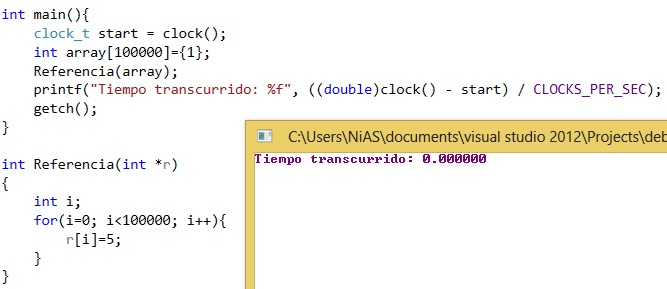
\includegraphics[scale=0.5]{Imagenes/7.jpg}\\
						POR REFERENCIA: Es notable que es más eficiente la ejecución al pasar un arreglo por referencia.\\
						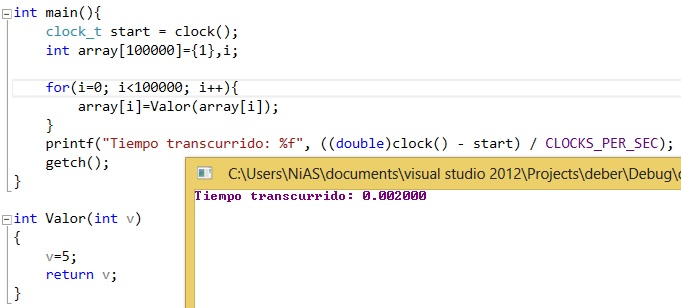
\includegraphics[scale=0.5]{Imagenes/8.jpg}\\
						POR VALOR: Se modificó la función para que hiciera lo mismo que la anterior, y notamos un cambio en los tiempos pero pasando cada elemento del arreglo por valor.
					\end{center}
					
			\end{itemize}


% Continuar con los siguientes capítulos y ejercicios:
% Ch6: 1, 2, 7
% Ch7: 1 - 6, 9
% Ch8: 3, 4, 5
% Ch9: 1, 5
% Recuerden que todos corresponden a las secciones de "Programming Exercises".

\end{document}
